\subsection{External Memory}

\subsubsection{Hard Disk Drives (HDD) - Magnetic Disks}

\begin{figure}[H]
    \centering
    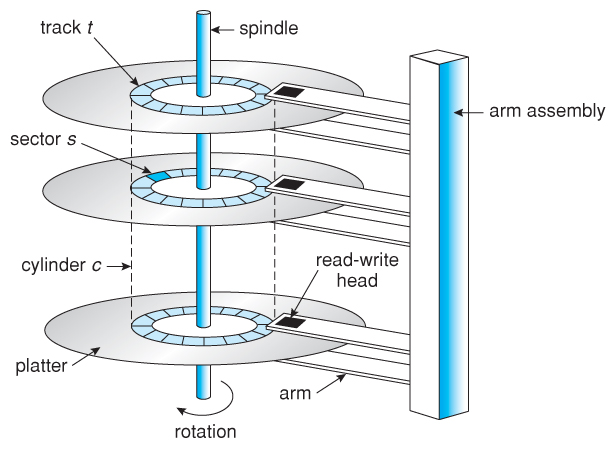
\includegraphics[width=0.58\textwidth]{chaps/memory/external-memory/hdd-layout.jpg}
    \caption{Disk Data Layout}
\end{figure}

\emph{Terminologies about the HDD layout and components}
\begin{itemize}
    \item \textbf{Platter}: Magnetically coated disks.
    \item \textbf{Track}: Concentric rings on a platter.
    \item \textbf{Sector}: A segment of a track, usually 512 bytes.
    \item \textbf{Cylinder}: Tracks of different platters that are under the read/write head
        at the same time.
\end{itemize}

\emph{Formats of Tracks}

Tracks contain sectors that hold data and other bits that
are useful for the disk controller. The example of a track format can be:
\begin{itemize}
    \item Each track contains 30 sectors of fixed-length 600 bytes, with 512 bytes for data
        and 88 bytes for control information.
    \item Each sector contains several fields: \begin{itemize}
        \item \textbf{Gap 1} (17 bytes): Used to separate sectors.
        \item \textbf{ID Field}: Contains Synch (1 byte), Track, Head, Sector \# (4 bytes),
            and CRC (2 bytes).
        \item \textbf{Gap 2} (41 bytes): Used to separate ID field and data field.
        \item \textbf{Data Field} (515 bytes): Contains 1 Synch byte, 512 bytes of data, and 2
            CRC bytes.
        \item \textbf{Gap 3} (40 bytes)
    \end{itemize}
\end{itemize}

\begin{figure}[H]
    \centering
    \begin{subfigure}{0.28\textwidth}
        \centering
        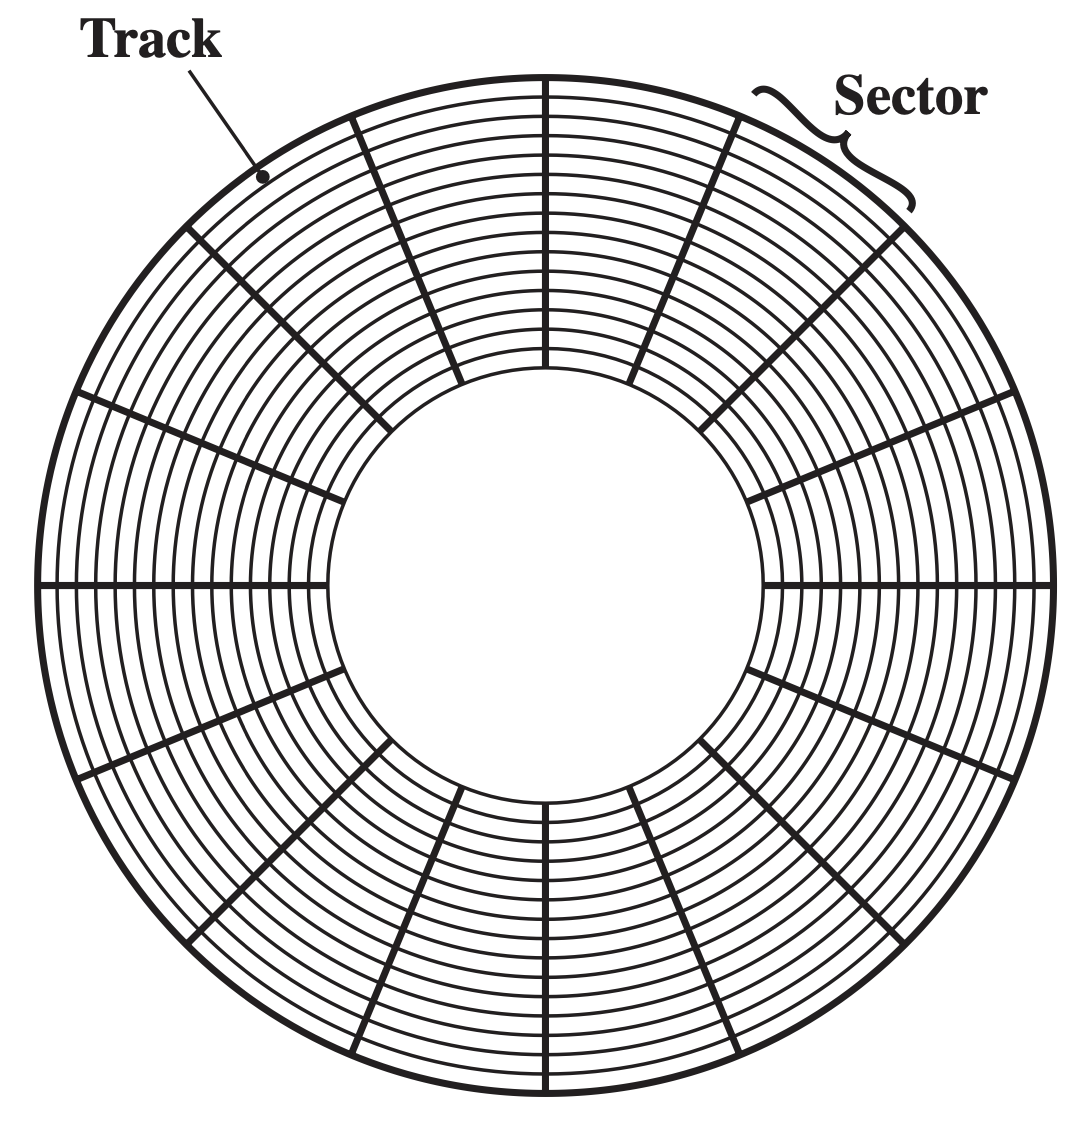
\includegraphics[width=\textwidth]{chaps/memory/external-memory/disk-layout-cav.png}
        \caption{CAV}
    \end{subfigure}
    \hspace{0.1\textwidth}
    \begin{subfigure}{0.28\textwidth}
        \centering
        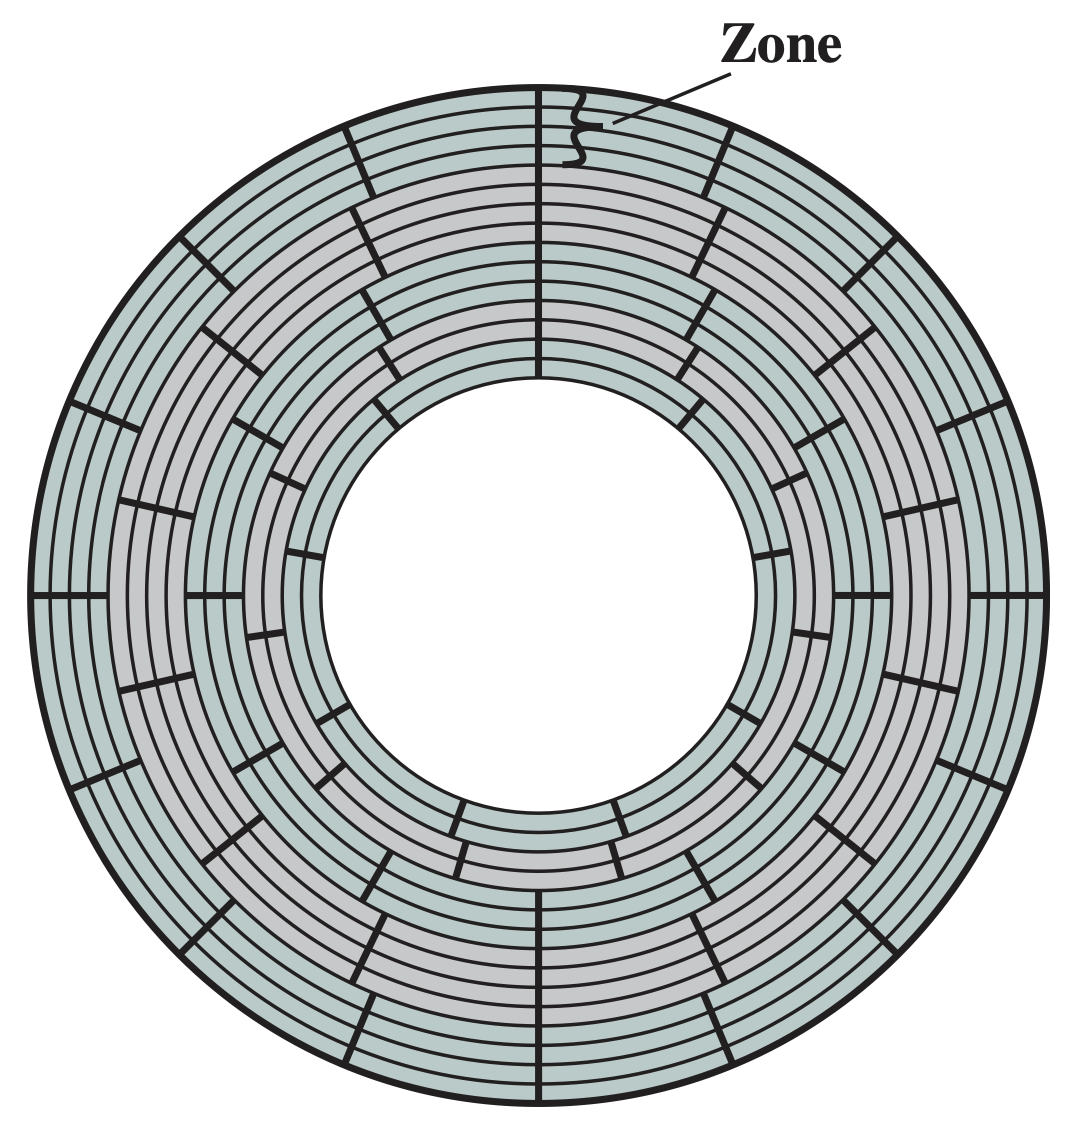
\includegraphics[width=\textwidth]{chaps/memory/external-memory/disk-layout-mzr.png}
        \caption{MZR}
    \end{subfigure}
    \caption{Disk Layout Methods}
\end{figure}

\emph{Disk Layout Methods}
\begin{itemize}
    \item \textbf{Constant Angular Velocity (CAV)}: Blocks of data can be directly addressed
        by track and sector. Read/write is easy. However, density of data decreases from the
        inner tracks to the outer tracks, which wastes space.
    \item \textbf{Multiple Zone Recording (MZR)}: Divides the disk into zones, with each zone
        having a different number of sectors per track. Note that the data density is not
        exactly the same, but only approximated to be the same. This allows maximised storage
        capacity.
\end{itemize}

\emph{Disk Access Time}

\begin{itemize}
    \item \textbf{Seek Time}: Move the read/write head from one cylinder to another.
        Depends on start and destination. Typical values: 5 - 15 ms (start up), 0.2 - 1 ms
        (consecutive tracks).
    \item \textbf{Rotational Latency}: Time for the required sector to rotate under the head.
        Average latency is the time for half a revolution.
        \begin{example}
            For a disk rotating at 7200 RPM, the average latency is given by: \[
                \frac{1}{7200 \text{ rotation minute}^{-1}}
                \times \frac{60\text{ s}}{1\text{ minute}}
                \times 1000 \text{ ms s}^{-1}
                \times \frac{1}{2} \text{ rotation} = \boxed{4.17 \text{ ms}}
            \]
        \end{example}
    \item \textbf{Data Transfer Time} ($t_T$): Typically, $t_T \ll \text{seek} + \text{latency}$.
        \[
            t_T = \frac{b}{N} \times \frac{1}{r} 
        \]
        where $b$ is bytes to be transfered, $N$ is bytes per track, and $r$ is the rotation
        speed in rps.
\end{itemize}

\subsubsection{Redundant Array of Independent Disks (RAID)}

\emph{Characteristics of RAID}

\begin{itemize}
    \item Several disk drives are arranged together and appear as one single disk to the operating
        system (a \textbf{logical disk}).
    \item Files are distributed in \textbf{strips} across the disks.
    \item Strips can be in physical blocks, sectors, or other units.
    \item RAID allows parallel operation.
    \item Redundant capacity stores parity information which guarantees 24/7 operation.
    \item Several levels, from RAID 0 to RAID 6.
\end{itemize}

\emph{RAID 0} {\normalfont\large (Non-redundant)}

\begin{itemize}
    \item Data is written in consecutive sectors in a round-robin fashion.
    \item Efficient for accessing a block of data.
    \item One disk failure will cause all strips to be lost without recovery.
\end{itemize}

\emph{RAID 1} {\normalfont\large (Mirroring)}

\begin{itemize}
    \item Fault tolerant, can recover from multi-disk failure as long as one copy still exists.
    \item During read, either copy can be used, hence reduce seek time.
    \item One logical write requires two physical writes, reduces write performance.
\end{itemize}

\emph{RAID 2}

\begin{itemize}
    \item Uses extra disks to store Error Correction Codes (Hamming codes), which is
        very expensive.
    \item Number of redundant disks $\approx \log_2 (\text{number of data disks})$.
    \item No commercial usage.
    \item Potential advantage: (when strip size is small) efficient for parallel read.
    \item Universally controlled spindles (all read/write heads move in parallel without
        individual control).
\end{itemize}

\emph{RAID 3} {\normalfont\large (Bit-interleaved Parity)}

\begin{itemize}
    \item One extra disk is used to store parity bit of the data disks.
    \item Can recover from one disk failure. Refer to Example \ref{ex:parity-bit-error-correction}
        for how parity bit can be used to recover data.
    \item Writing is also possible with one disk failure, use the above method to alter the
        parity bit.
    \item Error correction principle applies from RAID 3 to RAID 6.
\end{itemize}

\emph{RAID 4} {\normalfont\large (Block-level Parity)}

\begin{itemize}
    \item Similar to RAID 3, but parity is calculated on a block basis.
    \item Write to any block would result in the need of recauculating the parity block.
        Write penalty: 2 reads, 2 writes.
    \item Methods of writing: \begin{enumerate*}[label=(\arabic*)]
        \item Write data, recalculate parity, write parity; or
        \item Write data, compare old data with new data, add the difference to parity.
    \end{enumerate*}
    \item Individual spindle control.
    \item No commercial usage.
\end{itemize}

\emph{RAID 5} {\normalfont\large (Block-level Distributed Parity)}

\begin{itemize}
    \item Uses $(n-1)$ disks to store data.
    \item Difference from RAID 4: Parity is distributed across all disks.
    \item Difference from RAID 3: Parity is calculated on a block basis.
    \item Can endure one disk failure.
    \item Commonly used in Network Attached Storage (NAS).
\end{itemize}

\begin{figure}[H]
    \centering
    \hfill
    \begin{subfigure}{0.4\textwidth}
        \centering
        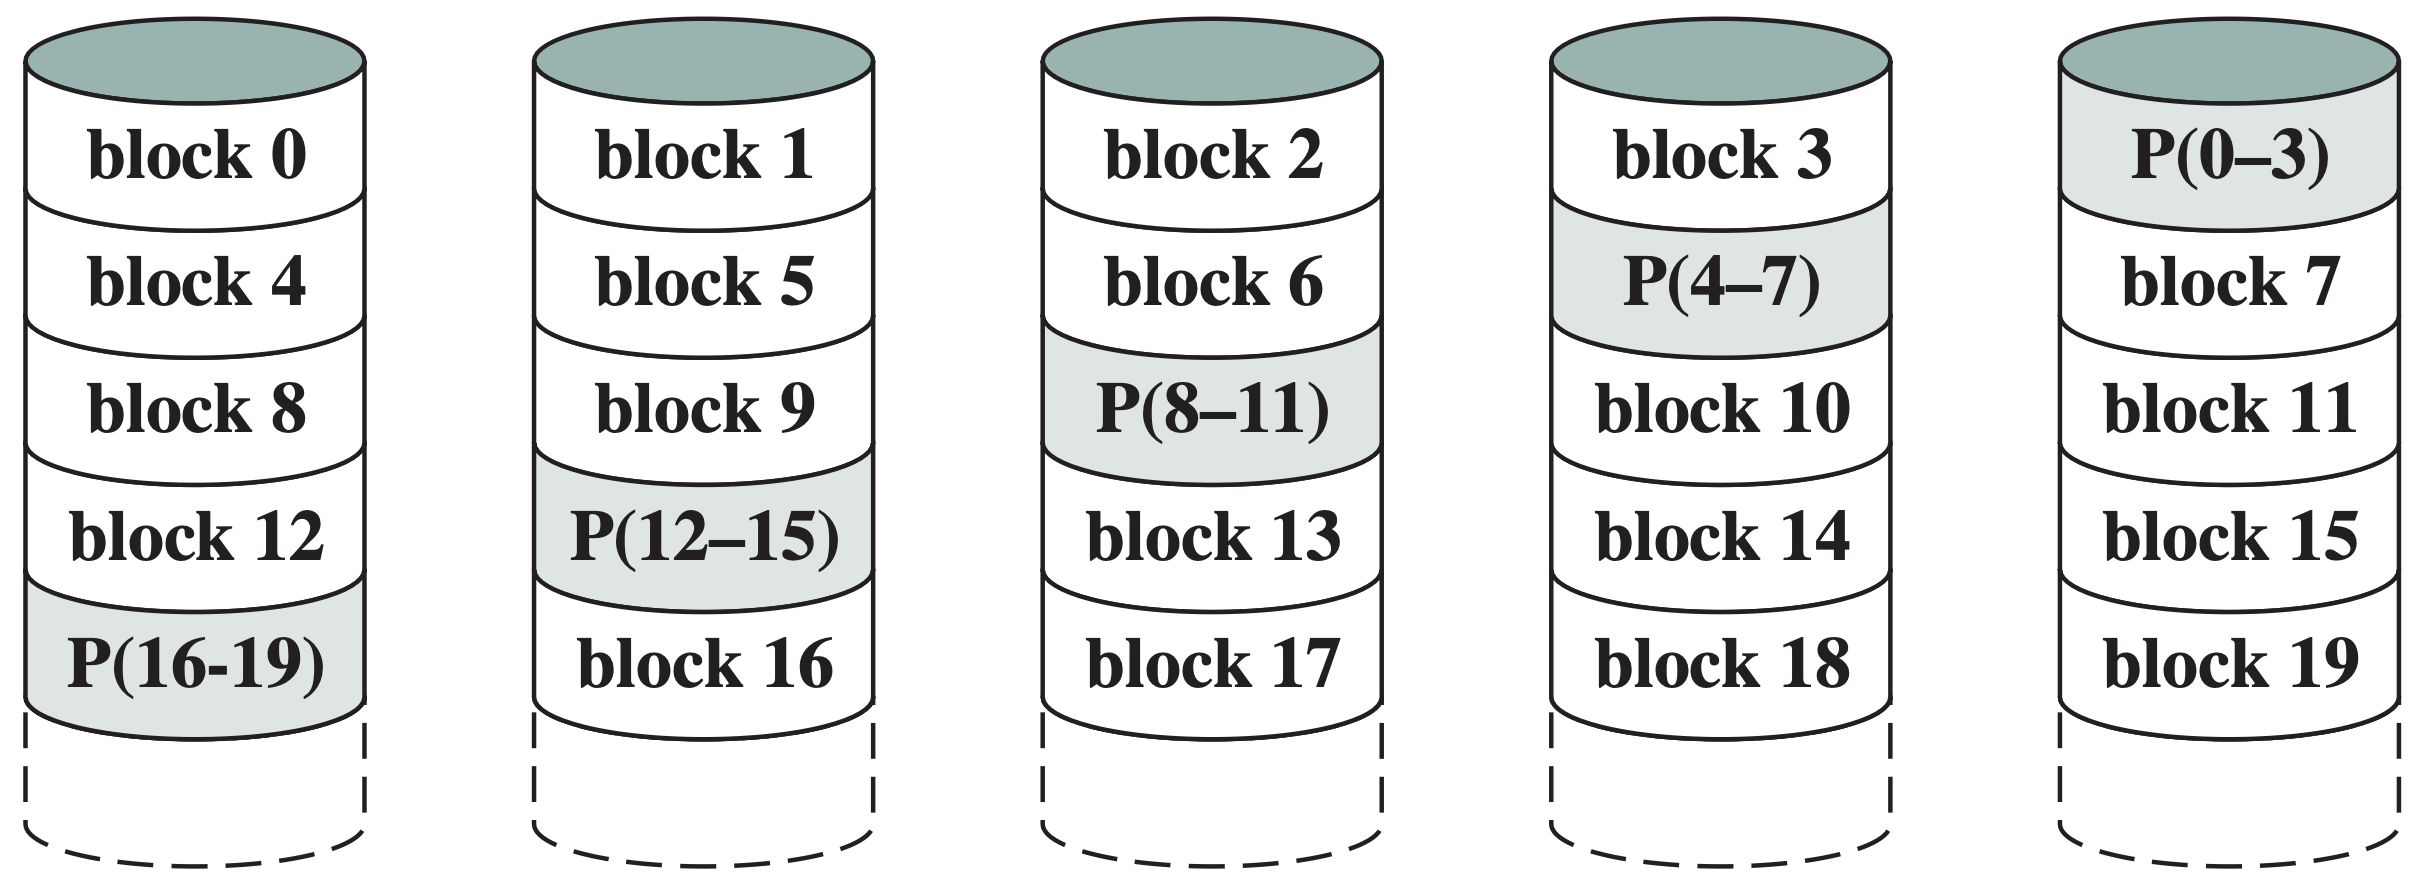
\includegraphics[width=\textwidth]{chaps/memory/external-memory/raid-level-5.png}
        \caption{RAID Level 5}
    \end{subfigure}
    \hfill
    \begin{subfigure}{0.5\textwidth}
        \centering
        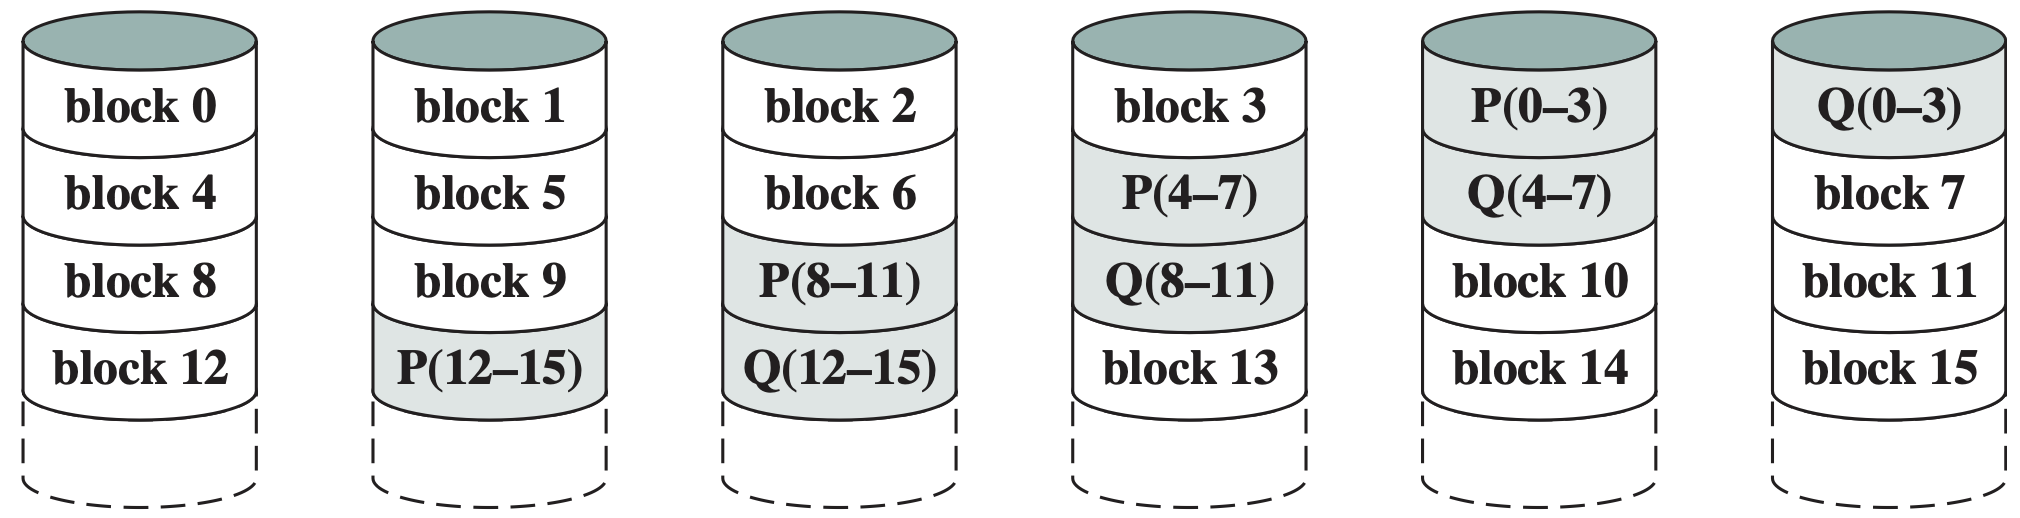
\includegraphics[width=\textwidth]{chaps/memory/external-memory/raid-level-6.png}
        \caption{RAID Level 6}
    \end{subfigure}
    \hfill
    \caption{Comparison between RAID 5 and RAID 6}
\end{figure}

\emph{RAID 6} {\normalfont\large (Dual Redundancy)}

\begin{itemize}
    \item Uses $(n-2)$ disks to store data.
    \item Similar to RAID 5, but uses two strips for parity, calculated by different methods.
    \item Parity distributed across different disks, require 2 extra disks.
    \item Can endure two disk failures.
\end{itemize}

\begin{table}[H]
    \centering
    \caption{Advantages and Disadvantages of Different RAID Levels}
    \begin{tabularx}{\textwidth}{|r|*{2}{>{\RaggedRight\arraybackslash}X|}}
        \hline
        \multicolumn{1}{|c|}{\textbf{Level}} & \multicolumn{1}{c|}{\textbf{Advantages}} & \multicolumn{1}{c|}{\textbf{Disadvantages}} \\
        \hline

        0 &

        % RAID 0 - Advantages
        I/O performance greatly improved by spreading data across disks. \par
        No parity calculation overhead. \par
        Very simple design \& easy to implement.
        
        &

        % RAID 0 - Disadvantages
        One drive failure will result in data in one array to be lost.
        
        \\ \hline

        1 &

        % RAID 1 - Advantages
        100\% redundancy, no rebuild necessary when disk fails. \par
        May sustain multiple simultaneous drive failures. \par
        Simplest RAID storage subsystem design.
        
        &

        % RAID 1 - Disadvantages
        Highest (100\%) disk overhead of all RAID types.
        
        \\ \hline

        2 &

        % RAID 2 - Advantages
        High data transfer rate. \par
        The higher transfer rate required, the better data disk to ECC disk ratio. \par
        Relatively simpler controller design than RAID 3-5.
        
        &

        % RAID 2 - Disadvantages
        Expensive. \par
        Very high data disk to ECC disk ratio with smaller word sizes.
        
        \\ \hline

        3 &

        % RAID 3 - Advantages
        Very high read/write data transfer rate. \par
        Disk failure has insignificant impact on throughput. \par
        Low ECC to data disk ratio, higher efficiency.

        &

        % RAID 3 - Disadvantages
        Controller design is faily complex.
        
        \\ \hline

        4 &

        % RAID 4 - Advantages
        Very high read data transfer rate. \par
        Low ECC to data disk ratio, higher efficiency.

        &

        % RAID 4 - Disadvantages
        Quite complex controller design. \par
        Worst write transaction rate and Write aggregate transfer rate. \par
        Difficult and inefficient data rebuild after disk failure.

        \\ \hline

        5 &

        % RAID 5 - Advantages
        Highest Read data transaction rate. \par
        Low ECC to data disk ratio, higher efficiency. \par
        Good aggregate transfer rate.

        &

        % RAID 5 - Disadvantages
        Most complex controller design. \par
        Difficult to rebuild data after disk failure as compared to RAID 1.

        \\ \hline

        6 &

        % RAID 6 - Advantages
        Provides highest data fault tolerance. \par
        Can sustain multiple simultaneous drive failures.

        &

        % RAID 6 - Disadvantages
        More complex controller design than RAID 5. \par
        Controller overhead to compute parity is extremely high.

        \\ \hline
        
    \end{tabularx}
\end{table}

\subsubsection{Solid State Drives (SSD)}

SSDs are non-volatile storage devices that are based on semiconductor technology. They
have limited write cycles, but are faster than HDDs.

Advantages of SDDs over HDDs:
\begin{itemize}
    \item Faster I/O operation performance.
    \item Lower power consumption, cooler and quieter.
    \item Longer lifespan -- no mechanical parts for read/write.
    \item Durability -- less susceptible to physical shock.
    \item Lower access time.
\end{itemize}